\subsection{Summary}
So far, we have studied the different ways to go through a kNN computation from a workflow point of view with three main steps.
The first step focuses on data preprocessing, either for selecting pivots for each partition or for projecting data from high dimension to low dimension.
The second step is in charge of data partitioning and organization in the partitions using distance based method or size based method. The last step of the workflow is to actually compute the kNN in one or two MapReduce jobs. Figure~\ref{workflow} summarizes the 
workflow we have gone through in this section and the techniques that are associated with each step.

%\begin{figure*}[t]
%\center
%\scalebox{0.35}{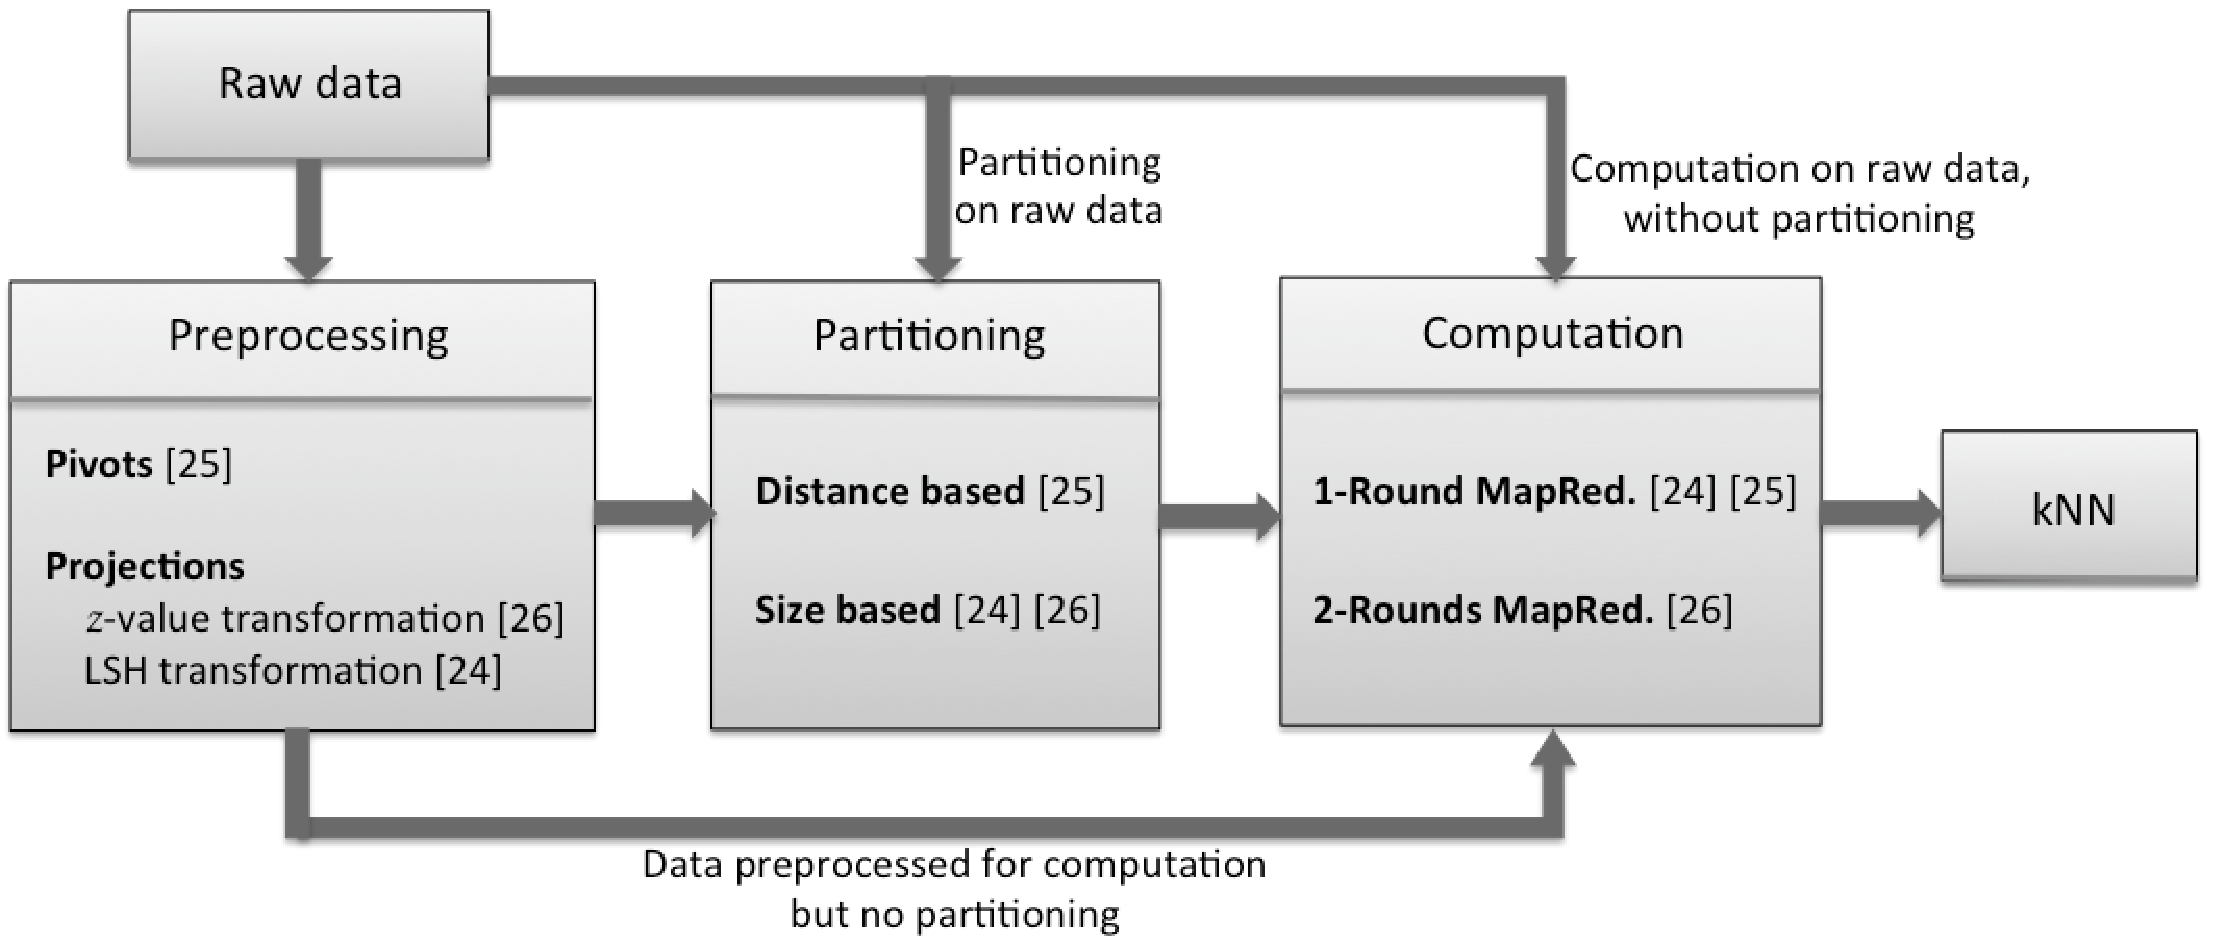
\includegraphics{res/workflow.pdf}}
%\caption{Usual workflow of a kNN computation using MapReduce \label{workflow}}
%\end{figure*}
